\section{Introduction}

Example s unit: fileName = showFileDialog(. . . );

We generate: /* Show file dialog and get file name */

Example s unit: if(saveAuctions())

We generate: /* If save auctions succeeds */


Real-world software development involves large source code repositories. 
Reading and trying to understand other people's code in such repositories 
is a difficult and unpleasant process for many software developers, 
especially when the code is not sufficiently commented.
For example, if the Java method in Fig.~\ref{figure:sourceCodeExample} doesn't 
have the comment on the first line, it will take quite some efforts for
even an experienced programmer to grasp the meaning of the code.
However, with a meaningful sentence such as 
``Returns true when one of the rows already contains all the pairs'' as
a descriptive comment, programmer's  productivity can be
tremendously improved.

\begin{figure}[th]
\begin{lstlisting}
// Returns true when one of the rows already contains all the pairs
  private static boolean isPartialRow(Iterable<ExpandedPair> pairs, Iterable<ExpandedRow> rows) {
    for (ExpandedRow r : rows) {
      boolean allFound = true;
      for (ExpandedPair p : pairs) {
        boolean found = false;
        for (ExpandedPair pp : r.getPairs()) {
          if (p.equals(pp)) {
            found = true;
            break;
          }
        }
        if (!found) {
          allFound = false;
          break;
        }
      }
      if (allFound) {
        return true;
      }
    }
    return false;
  }
\end{lstlisting}
%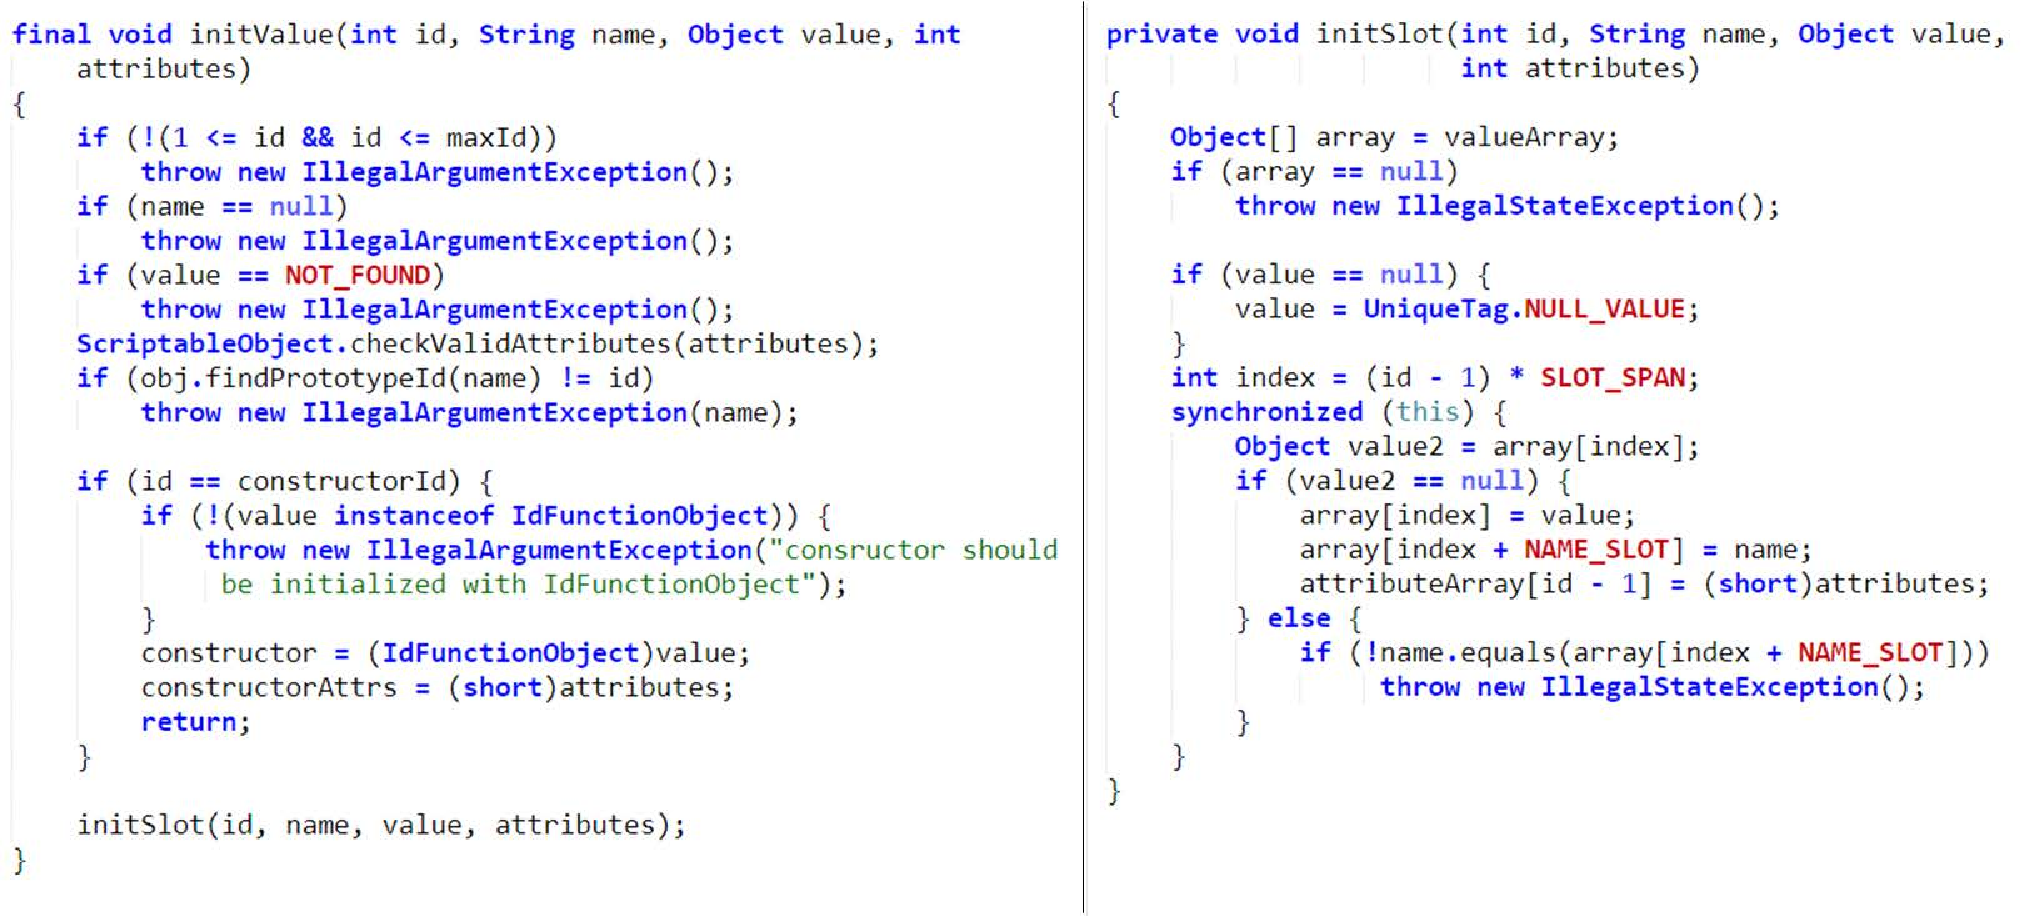
\includegraphics[width=16cm]{img/codeExample.pdf}
\caption{\label{figure:sourceCodeExample}source code example}
\end{figure}


A related scenario happens when one wants to search for a piece of code with
a specific functionality or meaning. Ordinary keyword search would not work
because expressions in programs can be quite different from natural languages.
If methods have meaningful natural language comments, then
keyword matching or even semantic fuzzy search can be achieved.

Finally, code pieces which look quite different on the surface, due to
the use of different identifier names and different code structures,
may actually serve the same purpose.
Detecting duplicated or similar code fragments in a large repository
is a common software engineering practice that simplifies the maintenance
efforts and lowers development costs. Again, if all code pieces are sufficiently
commented, similar pieces can be detected by comparing their comments.

To automatically generate descriptive comments from source code, 
one needs a way of accurately representing the semantics of code blocks. 
One potential solution is to treat each code block as a document
and represent it by a topic distribution using models such as LDA. 
However, topic models, when applied in source code, 
have several limitations:

\begin{itemize}
\item a topic model treats documents as a bag of words and ignores the
structural information such as programming language syntax and
function or method calls in the code;
\item the contribution of lexical semantics to the meaning of code
is exaggerated;
\item comments produced can only be words but not phrases or sentences.
\end{itemize}

\KZ{One step toward making the generated comments more readible is to 
use templates to generate comments \cite{}. Give some descriptions of
such approach and its limitations. Give examples here to show why they
are not good enough.}

\KZ{State the challenges in our problem.}

Because of these reasons, in this paper, we use Recursive Neural Network (RNN) to combine the semantic and structural information from code.
Recursive Neural Network has been used in NLP field before, such as by
R. Socher et al.~\cite{socher2011parsing, socher2011semi} and by
O. Irsoy and C. Cardie~\cite{irsoy2014deep}.
This kind of RNN is based on the parse tree, so in NLP area researchers have to find the parse tree of natural sentences first, then use this RNN to train. Fig.~\ref{rnn:nlp} is a recursive neural network example in NLP, there are two sentences in this figure. In our problem, source codes have parse tree naturally, so Recursive Neural Network comes as a natural fit in our work.

\begin{figure}[h]
	\centering
	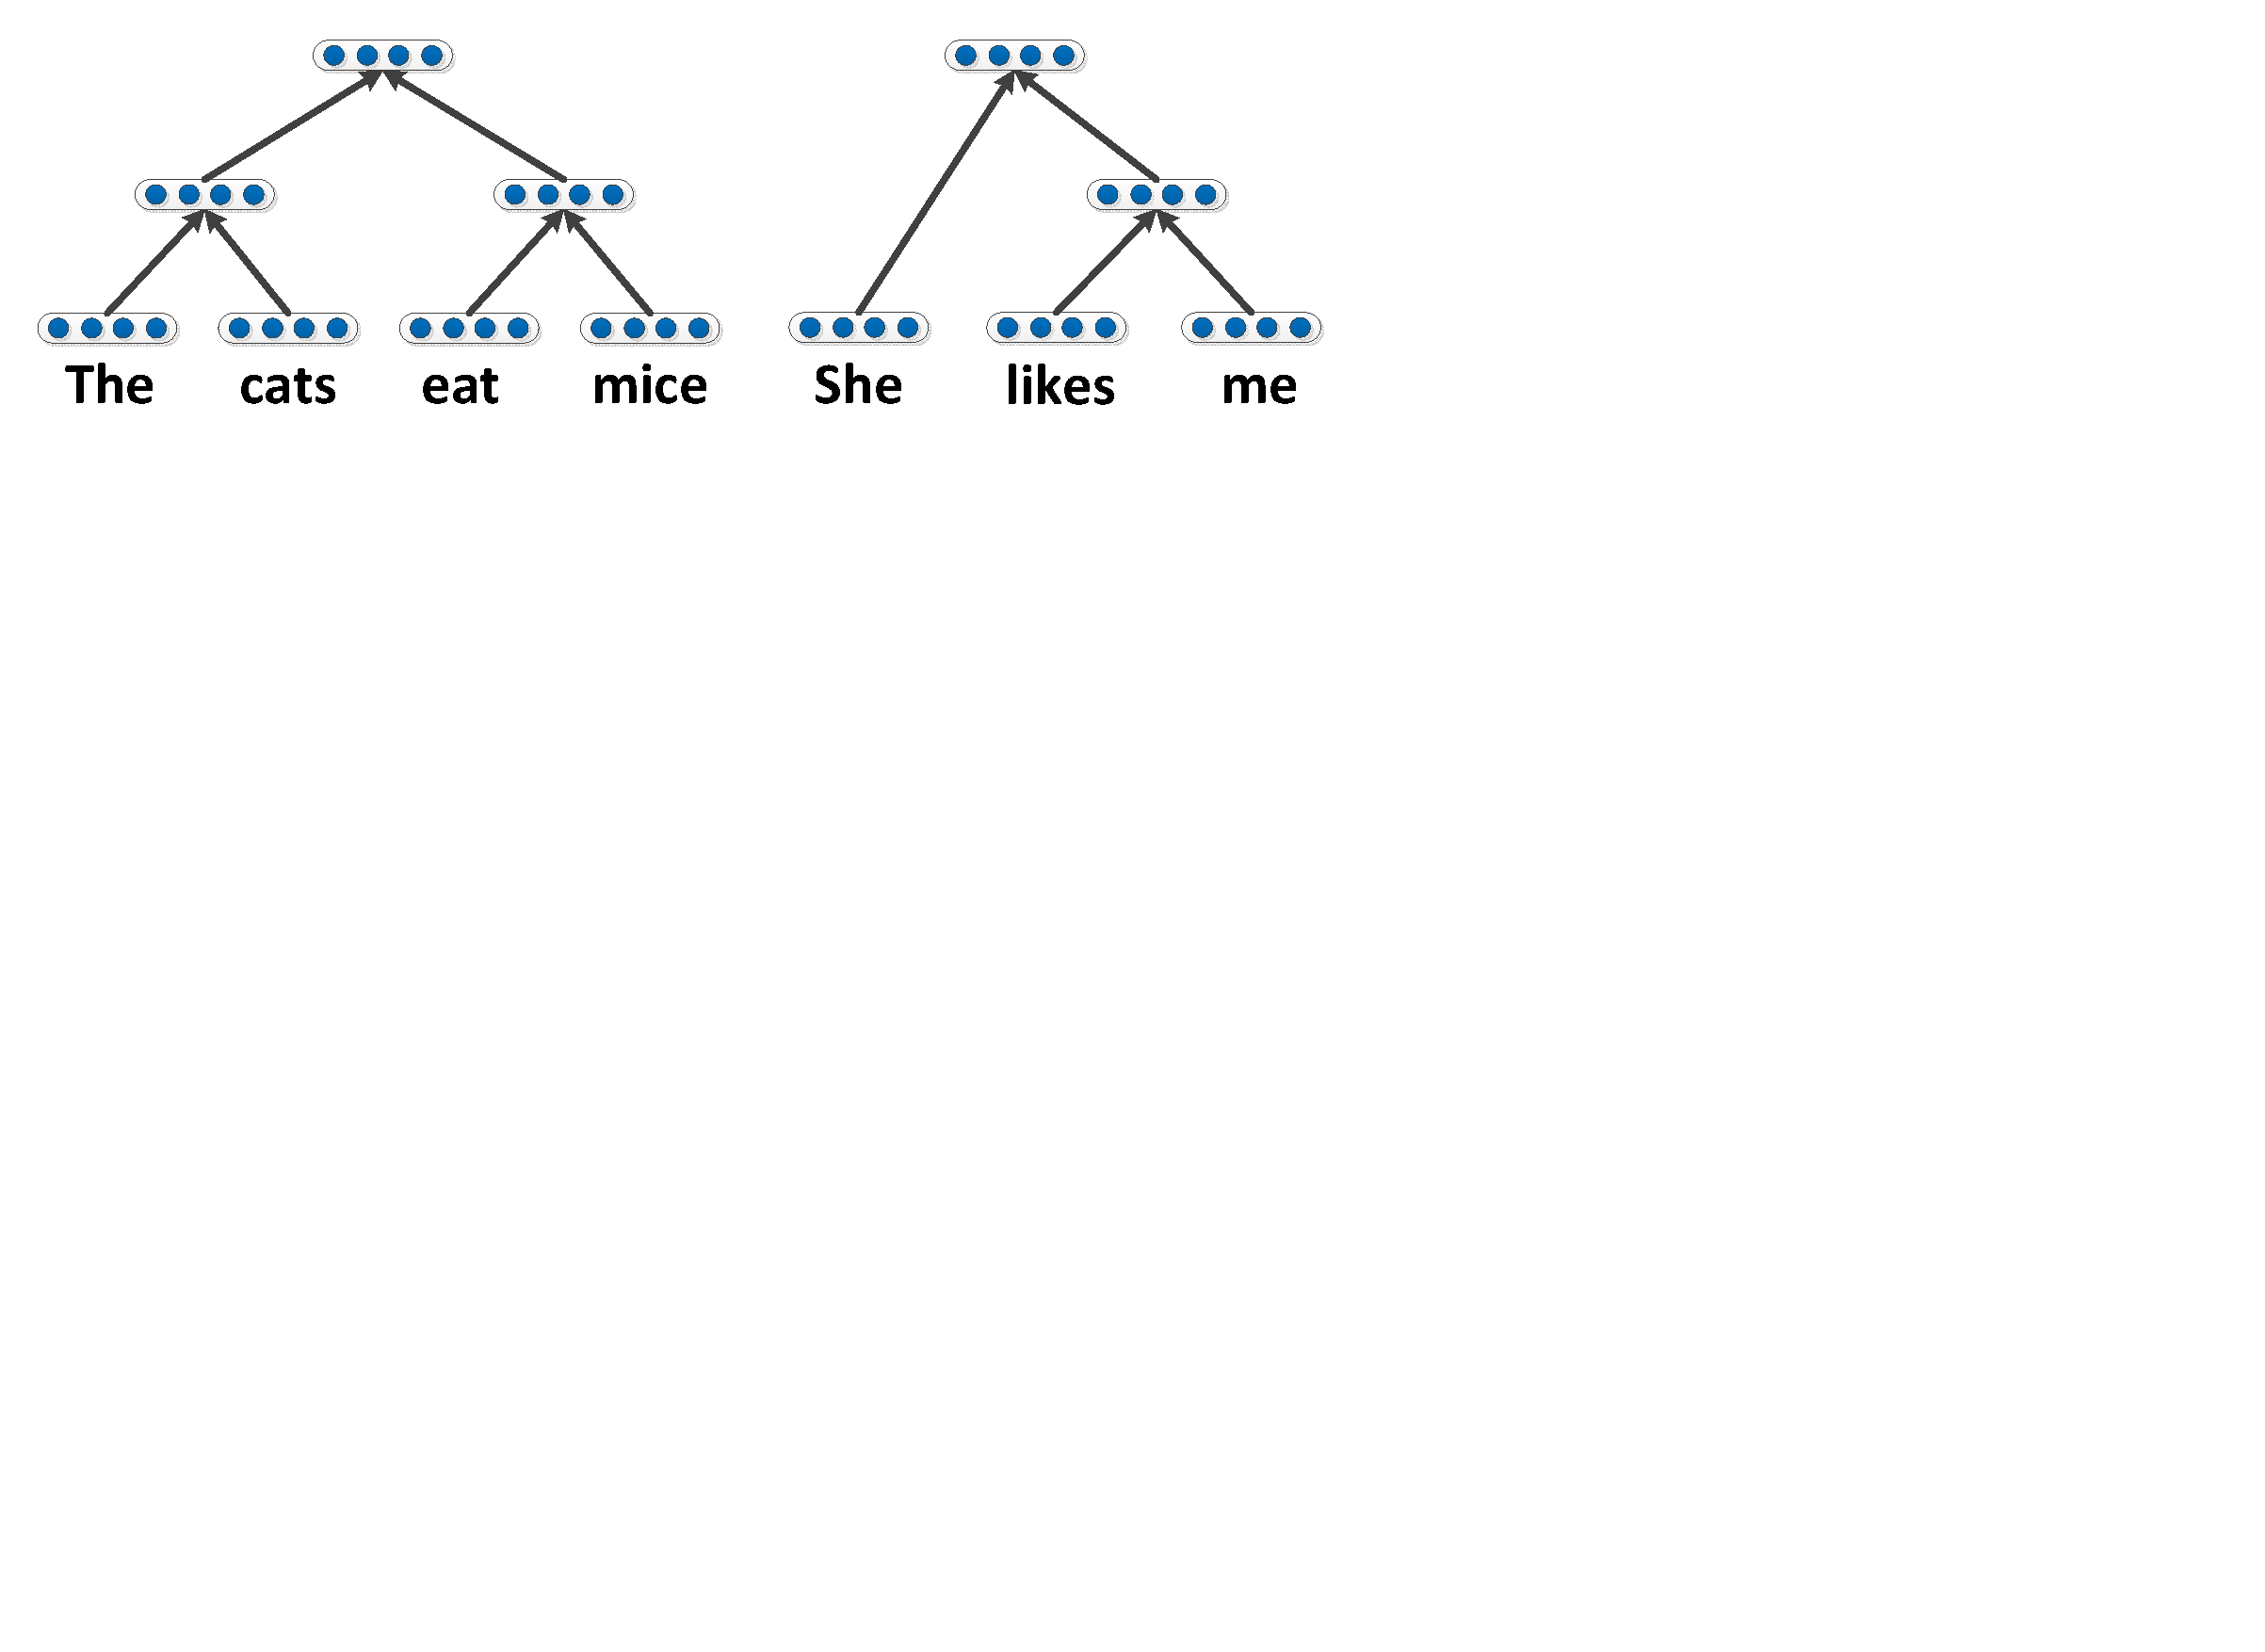
\includegraphics[width=\linewidth]{img/rnn_1.pdf}
	% where an .eps filename suffix will be assumed under latex,
	% and a .pdf suffix will be assumed for pdflatex; or what has been declared
	% via \DeclareGraphicsExtensions.
	\caption{Recursive Neural Network examples}
	\label{rnn:nlp}
\end{figure}

The parse trees in natural language process are all binary trees \KZ{This is
not true, dependency parse is not binary...} 
but the trees in source code are arbitrarily trees, so we design a new Recursive Neural Network called Code-RNN to extract the information of source code.

After using Code-RNN to train source code, we can get a vector representation of every method and this vector contains much information of source code, just like word embedding~\cite{mikolov2013distributed}. Then we choose the method that proposed by A. Karpathy and L. Fei-Fei~\cite{karpathy2015deep} and use these pre-trained vectors to learn how to generate comments significantly.

To make our model better at generating comments for project source code, we also add invocation information in our model when learning how to generate comments, so we totally make the following contributions to make our model work:
\KZ{Needs to rephrase the contributions}
\begin{itemize}
\item by designing a new Recursive Neural Network, \textbf{Code-RNN}, we strengthen the ability to describe {\em structural information}
of source code;
\item by adding method invocation information to the model,
we strengthen the ability to generate comments for other methods who have no manual comments;
\item by splitting one parse tree into many subtrees, we make the Code-RNN has the same depth for all methods.
\end{itemize}

Next, we first present our approach, as well as some evaluation results. We then
discuss some related work before concluding the paper.
